% REV00 Tue 04 May 2021 13:55:16 WIB
% START Tue 04 May 2021 13:55:16 WIB

\chapter{XXX}

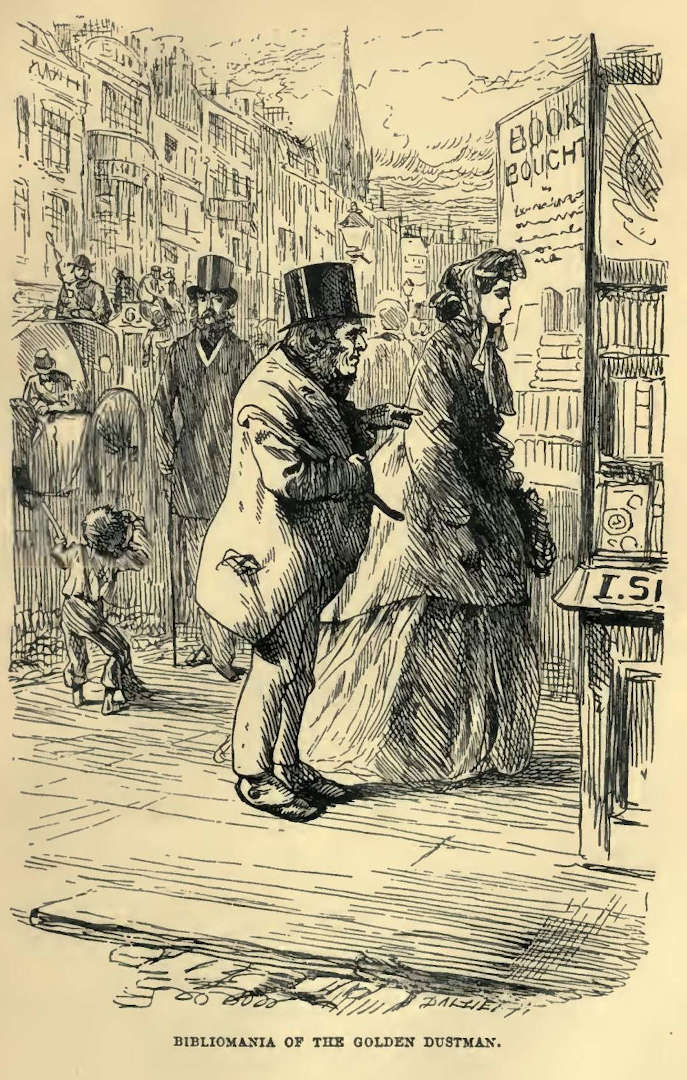
\includegraphics[scale=2.3]{03-05-01}

Chapter 5

CONCERNING THE MENDICANT’S BRIDE


The impressive gloom with which Mrs Wilfer received her husband on his
return from the wedding, knocked so hard at the door of the cherubic
conscience, and likewise so impaired the firmness of the cherubic legs,
that the culprit’s tottering condition of mind and body might have
roused suspicion in less occupied persons that the grimly heroic lady,
Miss Lavinia, and that esteemed friend of the family, Mr George Sampson.
But, the attention of all three being fully possessed by the main
fact of the marriage, they had happily none to bestow on the guilty
conspirator; to which fortunate circumstance he owed the escape for
which he was in nowise indebted to himself.

‘You do not, R. W.’ said Mrs Wilfer from her stately corner, ‘inquire
for your daughter Bella.’

‘To be sure, my dear,’ he returned, with a most flagrant assumption of
unconsciousness, ‘I did omit it. How--or perhaps I should rather say
where--IS Bella?’

‘Not here,’ Mrs Wilfer proclaimed, with folded arms.

The cherub faintly muttered something to the abortive effect of ‘Oh,
indeed, my dear!’

‘Not here,’ repeated Mrs Wilfer, in a stern sonorous voice. ‘In a word,
R. W., you have no daughter Bella.’

‘No daughter Bella, my dear?’

‘No. Your daughter Bella,’ said Mrs Wilfer, with a lofty air of never
having had the least copartnership in that young lady: of whom she now
made reproachful mention as an article of luxury which her husband had
set up entirely on his own account, and in direct opposition to her
advice: ‘--your daughter Bella has bestowed herself upon a Mendicant.’

‘Good gracious, my dear!’

‘Show your father his daughter Bella’s letter, Lavinia,’ said Mrs
Wilfer, in her monotonous Act of Parliament tone, and waving her hand.
‘I think your father will admit it to be documentary proof of what I
tell him. I believe your father is acquainted with his daughter Bella’s
writing. But I do not know. He may tell you he is not. Nothing will
surprise me.’

‘Posted at Greenwich, and dated this morning,’ said the Irrepressible,
flouncing at her father in handing him the evidence. ‘Hopes Ma won’t be
angry, but is happily married to Mr John Rokesmith, and didn’t mention
it beforehand to avoid words, and please tell darling you, and love
to me, and I should like to know what you’d have said if any other
unmarried member of the family had done it!’

He read the letter, and faintly exclaimed ‘Dear me!’

‘You may well say Dear me!’ rejoined Mrs Wilfer, in a deep tone. Upon
which encouragement he said it again, though scarcely with the success
he had expected; for the scornful lady then remarked, with extreme
bitterness: ‘You said that before.’

‘It’s very surprising. But I suppose, my dear,’ hinted the cherub, as he
folded the letter after a disconcerting silence, ‘that we must make the
best of it? Would you object to my pointing out, my dear, that Mr
John Rokesmith is not (so far as I am acquainted with him), strictly
speaking, a Mendicant.’

‘Indeed?’ returned Mrs Wilfer, with an awful air of politeness. ‘Truly
so? I was not aware that Mr John Rokesmith was a gentleman of landed
property. But I am much relieved to hear it.’

‘I doubt if you HAVE heard it, my dear,’ the cherub submitted with
hesitation.

‘Thank you,’ said Mrs Wilfer. ‘I make false statements, it appears? So
be it. If my daughter flies in my face, surely my husband may. The one
thing is not more unnatural than the other. There seems a fitness in the
arrangement. By all means!’ Assuming, with a shiver of resignation, a
deadly cheerfulness.

But, here the Irrepressible skirmished into the conflict, dragging the
reluctant form of Mr Sampson after her.

‘Ma,’ interposed the young lady, ‘I must say I think it would be much
better if you would keep to the point, and not hold forth about
people’s flying into people’s faces, which is nothing more nor less than
impossible nonsense.’

‘How!’ exclaimed Mrs Wilfer, knitting her dark brows.

‘Just im-possible nonsense, Ma,’ returned Lavvy, ‘and George Sampson
knows it is, as well as I do.’

Mrs Wilfer suddenly becoming petrified, fixed her indignant eyes upon
the wretched George: who, divided between the support due from him to
his love, and the support due from him to his love’s mamma, supported
nobody, not even himself.

‘The true point is,’ pursued Lavinia, ‘that Bella has behaved in a most
unsisterly way to me, and might have severely compromised me with George
and with George’s family, by making off and getting married in this very
low and disreputable manner--with some pew-opener or other, I suppose,
for a bridesmaid--when she ought to have confided in me, and ought
to have said, “If, Lavvy, you consider it due to your engagement with
George, that you should countenance the occasion by being present, then
Lavvy, I beg you to BE present, keeping my secret from Ma and Pa.” As of
course I should have done.’

‘As of course you would have done? Ingrate!’ exclaimed Mrs Wilfer.
‘Viper!’

‘I say! You know ma’am. Upon my honour you mustn’t,’ Mr Sampson
remonstrated, shaking his head seriously, ‘With the highest respect for
you, ma’am, upon my life you mustn’t. No really, you know. When a man
with the feelings of a gentleman finds himself engaged to a young lady,
and it comes (even on the part of a member of the family) to vipers, you
know!--I would merely put it to your own good feeling, you know,’ said
Mr Sampson, in rather lame conclusion.

Mrs Wilfer’s baleful stare at the young gentleman in acknowledgment of
his obliging interference was of such a nature that Miss Lavinia burst
into tears, and caught him round the neck for his protection.

‘My own unnatural mother,’ screamed the young lady, ‘wants to annihilate
George! But you shan’t be annihilated, George. I’ll die first!’

Mr Sampson, in the arms of his mistress, still struggled to shake his
head at Mrs Wilfer, and to remark: ‘With every sentiment of respect for
you, you know, ma’am--vipers really doesn’t do you credit.’

‘You shall not be annihilated, George!’ cried Miss Lavinia. ‘Ma shall
destroy me first, and then she’ll be contented. Oh, oh, oh! Have I lured
George from his happy home to expose him to this! George, dear, be free!
Leave me, ever dearest George, to Ma and to my fate. Give my love to
your aunt, George dear, and implore her not to curse the viper that has
crossed your path and blighted your existence. Oh, oh, oh!’ The young
lady who, hysterically speaking, was only just come of age, and had
never gone off yet, here fell into a highly creditable crisis, which,
regarded as a first performance, was very successful; Mr Sampson,
bending over the body meanwhile, in a state of distraction, which
induced him to address Mrs Wilfer in the inconsistent expressions:
‘Demon--with the highest respect for you--behold your work!’

The cherub stood helplessly rubbing his chin and looking on, but on the
whole was inclined to welcome this diversion as one in which, by reason
of the absorbent properties of hysterics, the previous question would
become absorbed. And so, indeed, it proved, for the Irrepressible
gradually coming to herself; and asking with wild emotion, ‘George dear,
are you safe?’ and further, ‘George love, what has happened? Where is
Ma?’ Mr Sampson, with words of comfort, raised her prostrate form, and
handed her to Mrs Wilfer as if the young lady were something in the
nature of refreshments. Mrs Wilfer with dignity partaking of the
refreshments, by kissing her once on the brow (as if accepting an
oyster), Miss Lavvy, tottering, returned to the protection of Mr
Sampson; to whom she said, ‘George dear, I am afraid I have been
foolish; but I am still a little weak and giddy; don’t let go my hand,
George!’ And whom she afterwards greatly agitated at intervals, by
giving utterance, when least expected, to a sound between a sob and a
bottle of soda water, that seemed to rend the bosom of her frock.

Among the most remarkable effects of this crisis may be mentioned its
having, when peace was restored, an inexplicable moral influence, of an
elevating kind, on Miss Lavinia, Mrs Wilfer, and Mr George Sampson, from
which R. W. was altogether excluded, as an outsider and non-sympathizer.
Miss Lavinia assumed a modest air of having distinguished herself; Mrs
Wilfer, a serene air of forgiveness and resignation; Mr Sampson, an air
of having been improved and chastened. The influence pervaded the spirit
in which they returned to the previous question.

‘George dear,’ said Lavvy, with a melancholy smile, ‘after what has
passed, I am sure Ma will tell Pa that he may tell Bella we shall all be
glad to see her and her husband.’

Mr Sampson said he was sure of it too; murmuring how eminently he
respected Mrs Wilfer, and ever must, and ever would. Never more
eminently, he added, than after what had passed.

‘Far be it from me,’ said Mrs Wilfer, making deep proclamation from her
corner, ‘to run counter to the feelings of a child of mine, and of a
Youth,’ Mr Sampson hardly seemed to like that word, ‘who is the object
of her maiden preference. I may feel--nay, know--that I have been
deluded and deceived. I may feel--nay, know--that I have been set
aside and passed over. I may feel--nay, know--that after having so far
overcome my repugnance towards Mr and Mrs Boffin as to receive them
under this roof, and to consent to your daughter Bella’s,’ here turning
to her husband, ‘residing under theirs, it were well if your daughter
Bella,’ again turning to her husband, ‘had profited in a worldly
point of view by a connection so distasteful, so disreputable. I may
feel--nay, know--that in uniting herself to Mr Rokesmith she has united
herself to one who is, in spite of shallow sophistry, a Mendicant. And
I may feel well assured that your daughter Bella,’ again turning to her
husband, ‘does not exalt her family by becoming a Mendicant’s bride. But
I suppress what I feel, and say nothing of it.’

Mr Sampson murmured that this was the sort of thing you might expect
from one who had ever in her own family been an example and never
an outrage. And ever more so (Mr Sampson added, with some degree of
obscurity,) and never more so, than in and through what had passed. He
must take the liberty of adding, that what was true of the mother
was true of the youngest daughter, and that he could never forget the
touching feelings that the conduct of both had awakened within him. In
conclusion, he did hope that there wasn’t a man with a beating heart who
was capable of something that remained undescribed, in consequence of
Miss Lavinia’s stopping him as he reeled in his speech.

‘Therefore, R. W.’ said Mrs Wilfer, resuming her discourse and turning
to her lord again, ‘let your daughter Bella come when she will, and she
will be received. So,’ after a short pause, and an air of having taken
medicine in it, ‘so will her husband.’

‘And I beg, Pa,’ said Lavinia, ‘that you will not tell Bella what I
have undergone. It can do no good, and it might cause her to reproach
herself.’

‘My dearest girl,’ urged Mr Sampson, ‘she ought to know it.’

‘No, George,’ said Lavinia, in a tone of resolute self-denial. ‘No,
dearest George, let it be buried in oblivion.’

Mr Sampson considered that, ‘too noble.’

‘Nothing is too noble, dearest George,’ returned Lavinia. ‘And Pa, I
hope you will be careful not to refer before Bella, if you can help
it, to my engagement to George. It might seem like reminding her of her
having cast herself away. And I hope, Pa, that you will think it equally
right to avoid mentioning George’s rising prospects, when Bella is
present. It might seem like taunting her with her own poor fortunes.
Let me ever remember that I am her younger sister, and ever spare her
painful contrasts, which could not but wound her sharply.’

Mr Sampson expressed his belief that such was the demeanour of Angels.
Miss Lavvy replied with solemnity, ‘No, dearest George, I am but too
well aware that I am merely human.’

Mrs Wilfer, for her part, still further improved the occasion by sitting
with her eyes fastened on her husband, like two great black notes of
interrogation, severely inquiring, Are you looking into your breast? Do
you deserve your blessings? Can you lay your hand upon your heart and
say that you are worthy of so hysterical a daughter? I do not ask you if
you are worthy of such a wife--put Me out of the question--but are
you sufficiently conscious of, and thankful for, the pervading moral
grandeur of the family spectacle on which you are gazing? These
inquiries proved very harassing to R. W. who, besides being a little
disturbed by wine, was in perpetual terror of committing himself by the
utterance of stray words that would betray his guilty foreknowledge.
However, the scene being over, and--all things considered--well over, he
sought refuge in a doze; which gave his lady immense offence.

‘Can you think of your daughter Bella, and sleep?’ she disdainfully
inquired.

To which he mildly answered, ‘Yes, I think I can, my dear.’

‘Then,’ said Mrs Wilfer, with solemn indignation, ‘I would recommend
you, if you have a human feeling, to retire to bed.’

‘Thank you, my dear,’ he replied; ‘I think it IS the best place for me.’
And with these unsympathetic words very gladly withdrew.

Within a few weeks afterwards, the Mendicant’s bride (arm-in-arm with
the Mendicant) came to tea, in fulfilment of an engagement made through
her father. And the way in which the Mendicant’s bride dashed at the
unassailable position so considerately to be held by Miss Lavy, and
scattered the whole of the works in all directions in a moment, was
triumphant.

‘Dearest Ma,’ cried Bella, running into the room with a radiant face,
‘how do you do, dearest Ma?’ And then embraced her, joyously. ‘And Lavvy
darling, how do YOU do, and how’s George Sampson, and how is he getting
on, and when are you going to be married, and how rich are you going
to grow? You must tell me all about it, Lavvy dear, immediately.
John, love, kiss Ma and Lavvy, and then we shall all be at home and
comfortable.’

Mrs Wilfer stared, but was helpless. Miss Lavinia stared, but was
helpless. Apparently with no compunction, and assuredly with no
ceremony, Bella tossed her bonnet away, and sat down to make the tea.

‘Dearest Ma and Lavvy, you both take sugar, I know. And Pa (you good
little Pa), you don’t take milk. John does. I didn’t before I was
married; but I do now, because John does. John dear, did you kiss Ma and
Lavvy? Oh, you did! Quite correct, John dear; but I didn’t see you do
it, so I asked. Cut some bread and butter, John; that’s a love. Ma likes
it doubled. And now you must tell me, dearest Ma and Lavvy, upon your
words and honours! Didn’t you for a moment--just a moment--think I was a
dreadful little wretch when I wrote to say I had run away?’

Before Mrs Wilfer could wave her gloves, the Mendicant’s bride in her
merriest affectionate manner went on again.

‘I think it must have made you rather cross, dear Ma and Lavvy, and I
know I deserved that you should be very cross. But you see I had been
such a heedless, heartless creature, and had led you so to expect that
I should marry for money, and so to make sure that I was incapable of
marrying for love, that I thought you couldn’t believe me. Because, you
see, you didn’t know how much of Good, Good, Good, I had learnt from
John. Well! So I was sly about it, and ashamed of what you supposed me
to be, and fearful that we couldn’t understand one another and might
come to words, which we should all be sorry for afterwards, and so I
said to John that if he liked to take me without any fuss, he might. And
as he did like, I let him. And we were married at Greenwich church in
the presence of nobody--except an unknown individual who dropped in,’
here her eyes sparkled more brightly, ‘and half a pensioner. And now,
isn’t it nice, dearest Ma and Lavvy, to know that no words have been
said which any of us can be sorry for, and that we are all the best of
friends at the pleasantest of teas!’

Having got up and kissed them again, she slipped back to her chair
(after a loop on the road to squeeze her husband round the neck) and
again went on.

‘And now you will naturally want to know, dearest Ma and Lavvy, how
we live, and what we have got to live upon. Well! And so we live on
Blackheath, in the charm--ingest of dolls’ houses, de--lightfully
furnished, and we have a clever little servant who is de--cidedly
pretty, and we are economical and orderly, and do everything by
clockwork, and we have a hundred and fifty pounds a year, and we
have all we want, and more. And lastly, if you would like to know in
confidence, as perhaps you may, what is my opinion of my husband, my
opinion is--that I almost love him!’

‘And if you would like to know in confidence, as perhaps you may,’
said her husband, smiling, as he stood by her side, without her having
detected his approach, ‘my opinion of my wife, my opinion is--.’ But
Bella started up, and put her hand upon his lips.

‘Stop, Sir! No, John, dear! Seriously! Please not yet a while! I want to
be something so much worthier than the doll in the doll’s house.’

‘My darling, are you not?’

‘Not half, not a quarter, so much worthier as I hope you may some
day find me! Try me through some reverse, John--try me through some
trial--and tell them after THAT, what you think of me.’

‘I will, my Life,’ said John. ‘I promise it.’

‘That’s my dear John. And you won’t speak a word now; will you?’

‘And I won’t,’ said John, with a very expressive look of admiration
around him, ‘speak a word now!’

She laid her laughing cheek upon his breast to thank him, and said,
looking at the rest of them sideways out of her bright eyes: ‘I’ll go
further, Pa and Ma and Lavvy. John don’t suspect it--he has no idea of
it--but I quite love him!’

Even Mrs Wilfer relaxed under the influence of her married daughter, and
seemed in a majestic manner to imply remotely that if R. W. had been a
more deserving object, she too might have condescended to come down from
her pedestal for his beguilement. Miss Lavinia, on the other hand, had
strong doubts of the policy of the course of treatment, and whether it
might not spoil Mr Sampson, if experimented on in the case of that young
gentleman. R. W. himself was for his part convinced that he was father
of one of the most charming of girls, and that Rokesmith was the most
favoured of men; which opinion, if propounded to him, Rokesmith would
probably not have contested.

The newly-married pair left early, so that they might walk at leisure to
their starting-place from London, for Greenwich. At first they were
very cheerful and talked much; but after a while, Bella fancied that her
husband was turning somewhat thoughtful. So she asked him:

‘John dear, what’s the matter?’

‘Matter, my love?’

‘Won’t you tell me,’ said Bella, looking up into his face, ‘what you are
thinking of?’

‘There’s not much in the thought, my soul. I was thinking whether you
wouldn’t like me to be rich?’

‘You rich, John?’ repeated Bella, shrinking a little.

‘I mean, really rich. Say, as rich as Mr Boffin. You would like that?’

‘I should be almost afraid to try, John dear. Was he much the better for
his wealth? Was I much the better for the little part I once had in it?’

‘But all people are not the worse for riches, my own.’

‘Most people?’ Bella musingly suggested with raised eyebrows.

‘Nor even most people, it may be hoped. If you were rich, for instance,
you would have a great power of doing good to others.’

‘Yes, sir, for instance,’ Bella playfully rejoined; ‘but should I
exercise the power, for instance? And again, sir, for instance; should
I, at the same time, have a great power of doing harm to myself?’

Laughing and pressing her arm, he retorted: ‘But still, again for
instance; would you exercise that power?’

‘I don’t know,’ said Bella, thoughtfully shaking her head. ‘I hope not.
I think not. But it’s so easy to hope not and think not, without the
riches.’

‘Why don’t you say, my darling--instead of that phrase--being poor?’ he
asked, looking earnestly at her.

‘Why don’t I say, being poor! Because I am not poor. Dear John, it’s not
possible that you suppose I think we are poor?’

‘I do, my love.’

‘Oh John!’

‘Understand me, sweetheart. I know that I am rich beyond all wealth in
having you; but I think OF you, and think FOR you. In such a dress as
you are wearing now, you first charmed me, and in no dress could you
ever look, to my thinking, more graceful or more beautiful. But you have
admired many finer dresses this very day; and is it not natural that I
wish I could give them to you?’

‘It’s very nice that you should wish it, John. It brings these tears of
grateful pleasure into my eyes, to hear you say so with such tenderness.
But I don’t want them.’

‘Again,’ he pursued, ‘we are now walking through the muddy streets. I
love those pretty feet so dearly, that I feel as if I could not bear the
dirt to soil the sole of your shoe. Is it not natural that I wish you
could ride in a carriage?’

‘It’s very nice,’ said Bella, glancing downward at the feet in question,
‘to know that you admire them so much, John dear, and since you do, I
am sorry that these shoes are a full size too large. But I don’t want a
carriage, believe me.’

‘You would like one if you could have one, Bella?’

‘I shouldn’t like it for its own sake, half so well as such a wish for
it. Dear John, your wishes are as real to me as the wishes in the Fairy
story, that were all fulfilled as soon as spoken. Wish me everything
that you can wish for the woman you dearly love, and I have as good as
got it, John. I have better than got it, John!’

They were not the less happy for such talk, and home was not the less
home for coming after it. Bella was fast developing a perfect genius
for home. All the loves and graces seemed (her husband thought) to have
taken domestic service with her, and to help her to make home engaging.

Her married life glided happily on. She was alone all day, for, after an
early breakfast her husband repaired every morning to the City, and did
not return until their late dinner hour. He was ‘in a China house,’ he
explained to Bella: which she found quite satisfactory, without pursuing
the China house into minuter details than a wholesale vision of tea,
rice, odd-smelling silks, carved boxes, and tight-eyed people in more
than double-soled shoes, with their pigtails pulling their heads of
hair off, painted on transparent porcelain. She always walked with her
husband to the railroad, and was always there again to meet him; her old
coquettish ways a little sobered down (but not much), and her dress
as daintily managed as if she managed nothing else. But, John gone to
business and Bella returned home, the dress would be laid aside, trim
little wrappers and aprons would be substituted, and Bella, putting back
her hair with both hands, as if she were making the most business-like
arrangements for going dramatically distracted, would enter on the
household affairs of the day. Such weighing and mixing and chopping
and grating, such dusting and washing and polishing, such snipping
and weeding and trowelling and other small gardening, such making and
mending and folding and airing, such diverse arrangements, and above all
such severe study! For Mrs J. R., who had never been wont to do too much
at home as Miss B. W., was under the constant necessity of referring for
advice and support to a sage volume entitled The Complete British Family
Housewife, which she would sit consulting, with her elbows on the table
and her temples on her hands, like some perplexed enchantress poring
over the Black Art. This, principally because the Complete British
Housewife, however sound a Briton at heart, was by no means an expert
Briton at expressing herself with clearness in the British tongue,
and sometimes might have issued her directions to equal purpose in the
Kamskatchan language. In any crisis of this nature, Bella would suddenly
exclaim aloud, ‘Oh you ridiculous old thing, what do you mean by that?
You must have been drinking!’ And having made this marginal note, would
try the Housewife again, with all her dimples screwed into an expression
of profound research.

There was likewise a coolness on the part of the British Housewife,
which Mrs John Rokesmith found highly exasperating. She would say,
‘Take a salamander,’ as if a general should command a private to catch
a Tartar. Or, she would casually issue the order, ‘Throw in a handful--’
of something entirely unattainable. In these, the Housewife’s most
glaring moments of unreason, Bella would shut her up and knock her on
the table, apostrophising her with the compliment, ‘O you ARE a stupid
old Donkey! Where am I to get it, do you think?’

Another branch of study claimed the attention of Mrs John Rokesmith for
a regular period every day. This was the mastering of the newspaper, so
that she might be close up with John on general topics when John came
home. In her desire to be in all things his companion, she would have
set herself with equal zeal to master Algebra, or Euclid, if he had
divided his soul between her and either. Wonderful was the way in which
she would store up the City Intelligence, and beamingly shed it
upon John in the course of the evening; incidentally mentioning the
commodities that were looking up in the markets, and how much gold had
been taken to the Bank, and trying to look wise and serious over it
until she would laugh at herself most charmingly and would say, kissing
him: ‘It all comes of my love, John dear.’

For a City man, John certainly did appear to care as little as might be
for the looking up or looking down of things, as well as for the gold
that got taken to the Bank. But he cared, beyond all expression, for his
wife, as a most precious and sweet commodity that was always looking up,
and that never was worth less than all the gold in the world. And she,
being inspired by her affection, and having a quick wit and a fine ready
instinct, made amazing progress in her domestic efficiency, though,
as an endearing creature, she made no progress at all. This was her
husband’s verdict, and he justified it by telling her that she had begun
her married life as the most endearing creature that could possibly be.

‘And you have such a cheerful spirit!’ he said, fondly. ‘You are like a
bright light in the house.’

‘Am I truly, John?’

‘Are you truly? Yes, indeed. Only much more, and much better.’

‘Do you know, John dear,’ said Bella, taking him by a button of his
coat, ‘that I sometimes, at odd moments--don’t laugh, John, please.’

Nothing should induce John to do it, when she asked him not to do it.

‘--That I sometimes think, John, I feel a little serious.’

‘Are you too much alone, my darling?’

‘O dear, no, John! The time is so short that I have not a moment too
much in the week.’

‘Why serious, my life, then? When serious?’

‘When I laugh, I think,’ said Bella, laughing as she laid her head upon
his shoulder. ‘You wouldn’t believe, sir, that I feel serious now? But I
do.’ And she laughed again, and something glistened in her eyes.

‘Would you like to be rich, pet?’ he asked her coaxingly.

‘Rich, John! How CAN you ask such goose’s questions?’

‘Do you regret anything, my love?’

‘Regret anything? No!’ Bella confidently answered. But then, suddenly
changing, she said, between laughing and glistening: ‘Oh yes, I do
though. I regret Mrs Boffin.’

‘I, too, regret that separation very much. But perhaps it is only
temporary. Perhaps things may so fall out, as that you may sometimes see
her again--as that we may sometimes see her again.’ Bella might be very
anxious on the subject, but she scarcely seemed so at the moment. With
an absent air, she was investigating that button on her husband’s coat,
when Pa came in to spend the evening.

Pa had his special chair and his special corner reserved for him on
all occasions, and--without disparagement of his domestic joys--was far
happier there, than anywhere. It was always pleasantly droll to see Pa
and Bella together; but on this present evening her husband thought her
more than usually fantastic with him.

‘You are a very good little boy,’ said Bella, ‘to come unexpectedly,
as soon as you could get out of school. And how have they used you at
school to-day, you dear?’

‘Well, my pet,’ replied the cherub, smiling and rubbing his hands as she
sat him down in his chair, ‘I attend two schools. There’s the Mincing
Lane establishment, and there’s your mother’s Academy. Which might you
mean, my dear?’

‘Both,’ said Bella.

‘Both, eh? Why, to say the truth, both have taken a little out of me
to-day, my dear, but that was to be expected. There’s no royal road to
learning; and what is life but learning!’

‘And what do you do with yourself when you have got your learning by
heart, you silly child?’

‘Why then, my dear,’ said the cherub, after a little consideration, ‘I
suppose I die.’

‘You are a very bad boy,’ retorted Bella, ‘to talk about dismal things
and be out of spirits.’

‘My Bella,’ rejoined her father, ‘I am not out of spirits. I am as gay
as a lark.’ Which his face confirmed.

‘Then if you are sure and certain it’s not you, I suppose it must be
I,’ said Bella; ‘so I won’t do so any more. John dear, we must give this
little fellow his supper, you know.’

‘Of course we must, my darling.’

‘He has been grubbing and grubbing at school,’ said Bella, looking at
her father’s hand and lightly slapping it, ‘till he’s not fit to be
seen. O what a grubby child!’

‘Indeed, my dear,’ said her father, ‘I was going to ask to be allowed to
wash my hands, only you find me out so soon.’

‘Come here, sir!’ cried Bella, taking him by the front of his coat,
‘come here and be washed directly. You are not to be trusted to do it
for yourself. Come here, sir!’

The cherub, to his genial amusement, was accordingly conducted to a
little washing-room, where Bella soaped his face and rubbed his face,
and soaped his hands and rubbed his hands, and splashed him and rinsed
him and towelled him, until he was as red as beet-root, even to his very
ears: ‘Now you must be brushed and combed, sir,’ said Bella, busily.
‘Hold the light, John. Shut your eyes, sir, and let me take hold of your
chin. Be good directly, and do as you are told!’

Her father being more than willing to obey, she dressed his hair in her
most elaborate manner, brushing it out straight, parting it, winding it
over her fingers, sticking it up on end, and constantly falling back on
John to get a good look at the effect of it. Who always received her
on his disengaged arm, and detained her, while the patient cherub stood
waiting to be finished.

‘There!’ said Bella, when she had at last completed the final touches.
‘Now, you are something like a genteel boy! Put your jacket on, and come
and have your supper.’

The cherub investing himself with his coat was led back to his
corner--where, but for having no egotism in his pleasant nature, he
would have answered well enough for that radiant though self-sufficient
boy, Jack Horner--Bella with her own hands laid a cloth for him, and
brought him his supper on a tray. ‘Stop a moment,’ said she, ‘we must
keep his little clothes clean;’ and tied a napkin under his chin, in a
very methodical manner.

While he took his supper, Bella sat by him, sometimes admonishing him
to hold his fork by the handle, like a polite child, and at other times
carving for him, or pouring out his drink. Fantastic as it all was, and
accustomed as she ever had been to make a plaything of her good father,
ever delighted that she should put him to that account, still there was
an occasional something on Bella’s part that was new. It could not be
said that she was less playful, whimsical, or natural, than she always
had been; but it seemed, her husband thought, as if there were some
rather graver reason than he had supposed for what she had so lately
said, and as if throughout all this, there were glimpses of an
underlying seriousness.

It was a circumstance in support of this view of the case, that when she
had lighted her father’s pipe, and mixed him his glass of grog, she sat
down on a stool between her father and her husband, leaning her arm upon
the latter, and was very quiet. So quiet, that when her father rose to
take his leave, she looked round with a start, as if she had forgotten
his being there.

‘You go a little way with Pa, John?’

‘Yes, my dear. Do you?’

‘I have not written to Lizzie Hexam since I wrote and told her that I
really had a lover--a whole one. I have often thought I would like to
tell her how right she was when she pretended to read in the live coals
that I would go through fire and water for him. I am in the humour to
tell her so to-night, John, and I’ll stay at home and do it.’

‘You are tired.’

‘Not at all tired, John dear, but in the humour to write to Lizzie. Good
night, dear Pa. Good night, you dear, good, gentle Pa!’

Left to herself she sat down to write, and wrote Lizzie a long letter.
She had but completed it and read it over, when her husband came back.
‘You are just in time, sir,’ said Bella; ‘I am going to give you your
first curtain lecture. It shall be a parlour-curtain lecture. You shall
take this chair of mine when I have folded my letter, and I will take
the stool (though you ought to take it, I can tell you, sir, if it’s
the stool of repentance), and you’ll soon find yourself taken to task
soundly.’

Her letter folded, sealed, and directed, and her pen wiped, and her
middle finger wiped, and her desk locked up and put away, and these
transactions performed with an air of severe business sedateness, which
the Complete British Housewife might have assumed, and certainly would
not have rounded off and broken down in with a musical laugh, as Bella
did: she placed her husband in his chair, and placed herself upon her
stool.

‘Now, sir! To begin at the beginning. What is your name?’

A question more decidedly rushing at the secret he was keeping from
her, could not have astounded him. But he kept his countenance and his
secret, and answered, ‘John Rokesmith, my dear.’

‘Good boy! Who gave you that name?’

With a returning suspicion that something might have betrayed him to
her, he answered, interrogatively, ‘My godfathers and my godmothers,
dear love?’

‘Pretty good!’ said Bella. ‘Not goodest good, because you hesitate about
it. However, as you know your Catechism fairly, so far, I’ll let you off
the rest. Now, I am going to examine you out of my own head. John dear,
why did you go back, this evening, to the question you once asked me
before--would I like to be rich?’

Again, his secret! He looked down at her as she looked up at him, with
her hands folded on his knee, and it was as nearly told as ever secret
was.

Having no reply ready, he could do no better than embrace her.

‘In short, dear John,’ said Bella, ‘this is the topic of my lecture: I
want nothing on earth, and I want you to believe it.’

‘If that’s all, the lecture may be considered over, for I do.’

‘It’s not all, John dear,’ Bella hesitated. ‘It’s only Firstly. There’s
a dreadful Secondly, and a dreadful Thirdly to come--as I used to say to
myself in sermon-time when I was a very small-sized sinner at church.’

‘Let them come, my dearest.’

‘Are you sure, John dear; are you absolutely certain in your innermost
heart of hearts--?’

‘Which is not in my keeping,’ he rejoined.

‘No, John, but the key is.--Are you absolutely certain that down at the
bottom of that heart of hearts, which you have given to me as I
have given mine to you, there is no remembrance that I was once very
mercenary?’

‘Why, if there were no remembrance in me of the time you speak of,’ he
softly asked her with his lips to hers, ‘could I love you quite as well
as I do; could I have in the Calendar of my life the brightest of its
days; could I whenever I look at your dear face, or hear your dear
voice, see and hear my noble champion? It can never have been that which
made you serious, darling?’

‘No John, it wasn’t that, and still less was it Mrs Boffin, though I
love her. Wait a moment, and I’ll go on with the lecture. Give me a
moment, because I like to cry for joy. It’s so delicious, John dear, to
cry for joy.’

She did so on his neck, and, still clinging there, laughed a little when
she said, ‘I think I am ready now for Thirdly, John.’

‘I am ready for Thirdly,’ said John, ‘whatever it is.’

‘I believe, John,’ pursued Bella, ‘that you believe that I believe--’

‘My dear child,’ cried her husband gaily, ‘what a quantity of
believing!’

‘Isn’t there?’ said Bella, with another laugh. ‘I never knew such a
quantity! It’s like verbs in an exercise. But I can’t get on with less
believing. I’ll try again. I believe, dear John, that you believe that
I believe that we have as much money as we require, and that we want for
nothing.’

‘It is strictly true, Bella.’

‘But if our money should by any means be rendered not so much--if we
had to stint ourselves a little in purchases that we can afford to
make now--would you still have the same confidence in my being quite
contented, John?’

‘Precisely the same confidence, my soul.’

‘Thank you, John dear, thousands upon thousands of times. And I may take
it for granted, no doubt,’ with a little faltering, ‘that you would be
quite as contented yourself John? But, yes, I know I may. For, knowing
that I should be so, how surely I may know that you would be so; you who
are so much stronger, and firmer, and more reasonable and more generous,
than I am.’

‘Hush!’ said her husband, ‘I must not hear that. You are all wrong
there, though otherwise as right as can be. And now I am brought to a
little piece of news, my dearest, that I might have told you earlier
in the evening. I have strong reason for confidently believing that
we shall never be in the receipt of a smaller income than our present
income.’

She might have shown herself more interested in the intelligence;
but she had returned to the investigation of the coat-button that had
engaged her attention a few hours before, and scarcely seemed to heed
what he said.

‘And now we have got to the bottom of it at last,’ cried her husband,
rallying her, ‘and this is the thing that made you serious?’

‘No dear,’ said Bella, twisting the button and shaking her head, ‘it
wasn’t this.’

‘Why then, Lord bless this little wife of mine, there’s a Fourthly!’
exclaimed John.

‘This worried me a little, and so did Secondly,’ said Bella, occupied
with the button, ‘but it was quite another sort of seriousness--a much
deeper and quieter sort of seriousness--that I spoke of John dear.’

As he bent his face to hers, she raised hers to meet it, and laid her
little right hand on his eyes, and kept it there.

‘Do you remember, John, on the day we were married, Pa’s speaking of the
ships that might be sailing towards us from the unknown seas?’

‘Perfectly, my darling!’

‘I think...among them...there is a ship upon the ocean...bringing...to
you and me...a little baby, John.’



